\documentclass[11pt]{article}

\usepackage[margin=1in]{geometry}
\usepackage{booktabs}
\usepackage{amsmath}
\usepackage{amsthm}
\usepackage{hyperref}
\usepackage{graphicx}
\usepackage{xcolor}
\usepackage{tabularx}
\usepackage{ragged2e}
\newcolumntype{Y}{>{\RaggedRight\arraybackslash}X}

\newtheorem{proposition}{Proposition}

\title{Graph 12: Opinion Dynamics (Deffuant--Weisbuch) \\
\large Dependency Analysis, Method, and Results}
\author{DPCN Assignment 1 --- Opinion Network Formation}
\date{\today}

\begin{document}
\maketitle
\sloppy

\section{Why this figure matters}

This is the only figure in the project involving an actual \emph{dynamical
process}. Everything else -- missingness diagnostics, item variance, the
correlation network, row-centring -- is static description of a fixed dataset.
Since the course is \emph{Dynamical Processes on Complex Networks}, without
this figure the report is a static network analysis wearing a dynamics title.

\section{Dependency analysis}

Before any code was written, the question was whether this figure could be
produced independently or whether it was blocked on other team members'
deliverables. It decomposes into three required inputs.

\begin{center}
\begin{tabularx}{\linewidth}{l l Y}
\toprule
Required input & Status & Source \\
\midrule
Respondent opinions (seed) & Available & \texttt{dataset\_imputed.csv}, item \texttt{E03} \\
A graph connecting respondents & \textbf{Missing} & Had to be built (see \S3) \\
The DW simulation & \textbf{Missing} & Had to be written (see \S4) \\
\bottomrule
\end{tabularx}
\end{center}

A search of the repository confirmed no existing dynamics, $k$NN, or
respondent-network code of any kind. The respondent graph was therefore the
only genuine gap -- and every ingredient it needs was already present, since
\texttt{outputs/sanitised\_data/row\_centred\_data.csv} (91 respondents $\times$
60 items, row-centred) is precisely the matrix such a graph is built from.

\subsection{What this figure does \emph{not} depend on}

The important half of the dependency answer is what it can skip:

\begin{itemize}
  \item \textbf{No null models.} DW makes no significance claim, so no
        configuration model, rewiring, or permutation machinery is required.
  \item \textbf{No community detection.} Cluster counts come out of the
        dynamics itself, not from Louvain.
  \item \textbf{No threshold or percolation sweep.} This is the decisive one.
        The respondent graph is sparsified by $k$-nearest-neighbours with
        \emph{fixed} $k = 4$, not by a correlation threshold chosen from a
        sweep. Nothing therefore waits on a threshold-selection result.
  \item \textbf{No item correlation matrix and no structural balance.}
\end{itemize}

\textbf{Conclusion: no blocking dependency.} The figure was buildable
immediately from artifacts already in the repository.

\subsection{One non-technical caveat}
The checked-in \texttt{CLAUDE.md} nominally assigns \texttt{dynamics.py} to
Person~3 and the respondent-network code to Person~2. Nothing blocked this
work technically, but if a teammate is independently building a
respondent-graph module, the two should be reconciled before both land. This
is a coordination item, not a code dependency.

\section{The respondent network}

DW requires nodes that hold opinions. Since each opinion is one respondent's
answer to one item, the nodes must be \textbf{respondents}, not items -- this
is a different network from the 60-node item--item network built by
\texttt{src/pipeline.py}.

\subsection{Construction}
\begin{enumerate}
  \item Start from the row-centred $91 \times 60$ matrix. Centring matters
        here for the same reason it matters elsewhere: without it, two
        respondents look similar merely because both agree with everything.
  \item Compute the $91 \times 91$ Pearson correlation between respondents.
  \item For each respondent, connect to their $k = 4$ most similar peers, and
        symmetrise by union: an edge exists if \emph{either} endpoint ranks
        the other in its top four.
\end{enumerate}

Union rather than mutual $k$NN is deliberate. Mutual $k$NN is documented to
fragment this data badly, and a fragmented graph would inflate the final
cluster count for reasons having nothing to do with the confidence threshold
under study -- disconnected components cannot merge no matter how large
$\varepsilon$ becomes.

\subsection{Resulting properties}

\begin{center}
\begin{tabularx}{\linewidth}{l l Y}
\toprule
Property & Value & Reference value in \texttt{CLAUDE.md} \\
\midrule
Nodes & 91 & 86 \\
Edges & 298 & 286 \\
Connected components & 1 & 1 \\
Mean degree & 6.55 & --- \\
\bottomrule
\end{tabularx}
\end{center}

The node-count difference is expected and explained: the reference values
assume a filter dropping respondents with more than 12 missing items (leaving
86), which this project does not apply -- it retains all 91 non-empty
respondents and recovers their missing cells by ordinal regression instead.
The structurally important property, a \emph{single connected component}, is
reproduced.

\section{The model}

Opinions $x_i \in [0,1]$ are seeded from item \texttt{E03} (``Class attendance
should be compulsory for all courses'', the most contested Education item
after \texttt{E04}/\texttt{E02}, sample SD $= 1.12$), rescaled by
$s(x) = (x+2)/4$.

At each step an edge $(u,v)$ is drawn uniformly at random from the graph. If
the two opinions lie within the confidence threshold, both move toward each
other:
\begin{equation}
|x_u - x_v| < \varepsilon
\quad\Longrightarrow\quad
\begin{cases}
x_u \leftarrow x_u + \mu\,(x_v - x_u) \\
x_v \leftarrow x_v + \mu\,(x_u - x_v)
\end{cases}
\end{equation}
with $\mu = 0.5$, so both interacting nodes land on their midpoint. If the
opinions differ by $\varepsilon$ or more, nothing happens. Runs proceed for up
to 60{,}000 interactions, with early termination once the state stops
changing.

\paragraph{Parameters.} $\varepsilon$ swept from 0.05 to 0.60 in steps of
0.05; 20 repetitions per $\varepsilon$; final clusters counted by rounding
opinions to 2 decimals and taking unique values. Every run is seeded for
reproducibility.

\section{Results}

\begin{center}
\begin{tabular}{lccc}
\toprule
$\varepsilon$ & $k$NN graph (mean $\pm$ sd) & Complete graph & Jittered control \\
\midrule
0.05 & $5.00 \pm 0.00$ & $5.00 \pm 0.00$ & $35.95 \pm 2.67$ \\
0.10 & $5.00 \pm 0.00$ & $5.00 \pm 0.00$ & $26.35 \pm 2.41$ \\
0.15 & $5.00 \pm 0.00$ & $5.00 \pm 0.00$ & $21.05 \pm 2.44$ \\
0.20 & $5.00 \pm 0.00$ & $5.00 \pm 0.00$ & $14.20 \pm 2.52$ \\
0.25 & $5.00 \pm 0.00$ & $5.00 \pm 0.00$ & $8.95 \pm 2.80$ \\
\midrule
0.30 & $4.45 \pm 1.12$ & $2.45 \pm 0.50$ & $6.50 \pm 1.60$ \\
0.35 & $4.00 \pm 1.55$ & $2.00 \pm 0.00$ & $5.10 \pm 1.09$ \\
0.40 & $3.35 \pm 0.79$ & $2.00 \pm 0.00$ & $3.95 \pm 1.28$ \\
0.45 & $3.15 \pm 0.85$ & $2.25 \pm 0.43$ & $2.95 \pm 0.92$ \\
0.50 & $2.00 \pm 0.77$ & $2.05 \pm 0.22$ & $2.35 \pm 0.79$ \\
0.55 & $1.65 \pm 0.48$ & $1.95 \pm 0.22$ & $1.65 \pm 0.48$ \\
0.60 & $1.30 \pm 0.46$ & $1.65 \pm 0.48$ & $1.20 \pm 0.40$ \\
\bottomrule
\end{tabular}
\end{center}

The main ($k$NN) column tracks the project's frozen reference values closely:
5.0 clusters for $\varepsilon \le 0.25$ (exact), 4.45 vs.\ 4.2 at 0.30, 3.35
vs.\ 3.0 at 0.40, 2.00 vs.\ 1.6 at 0.50. Consensus is approached near
$\varepsilon \approx 0.55$--$0.60$.

\begin{figure}[h]
\centering
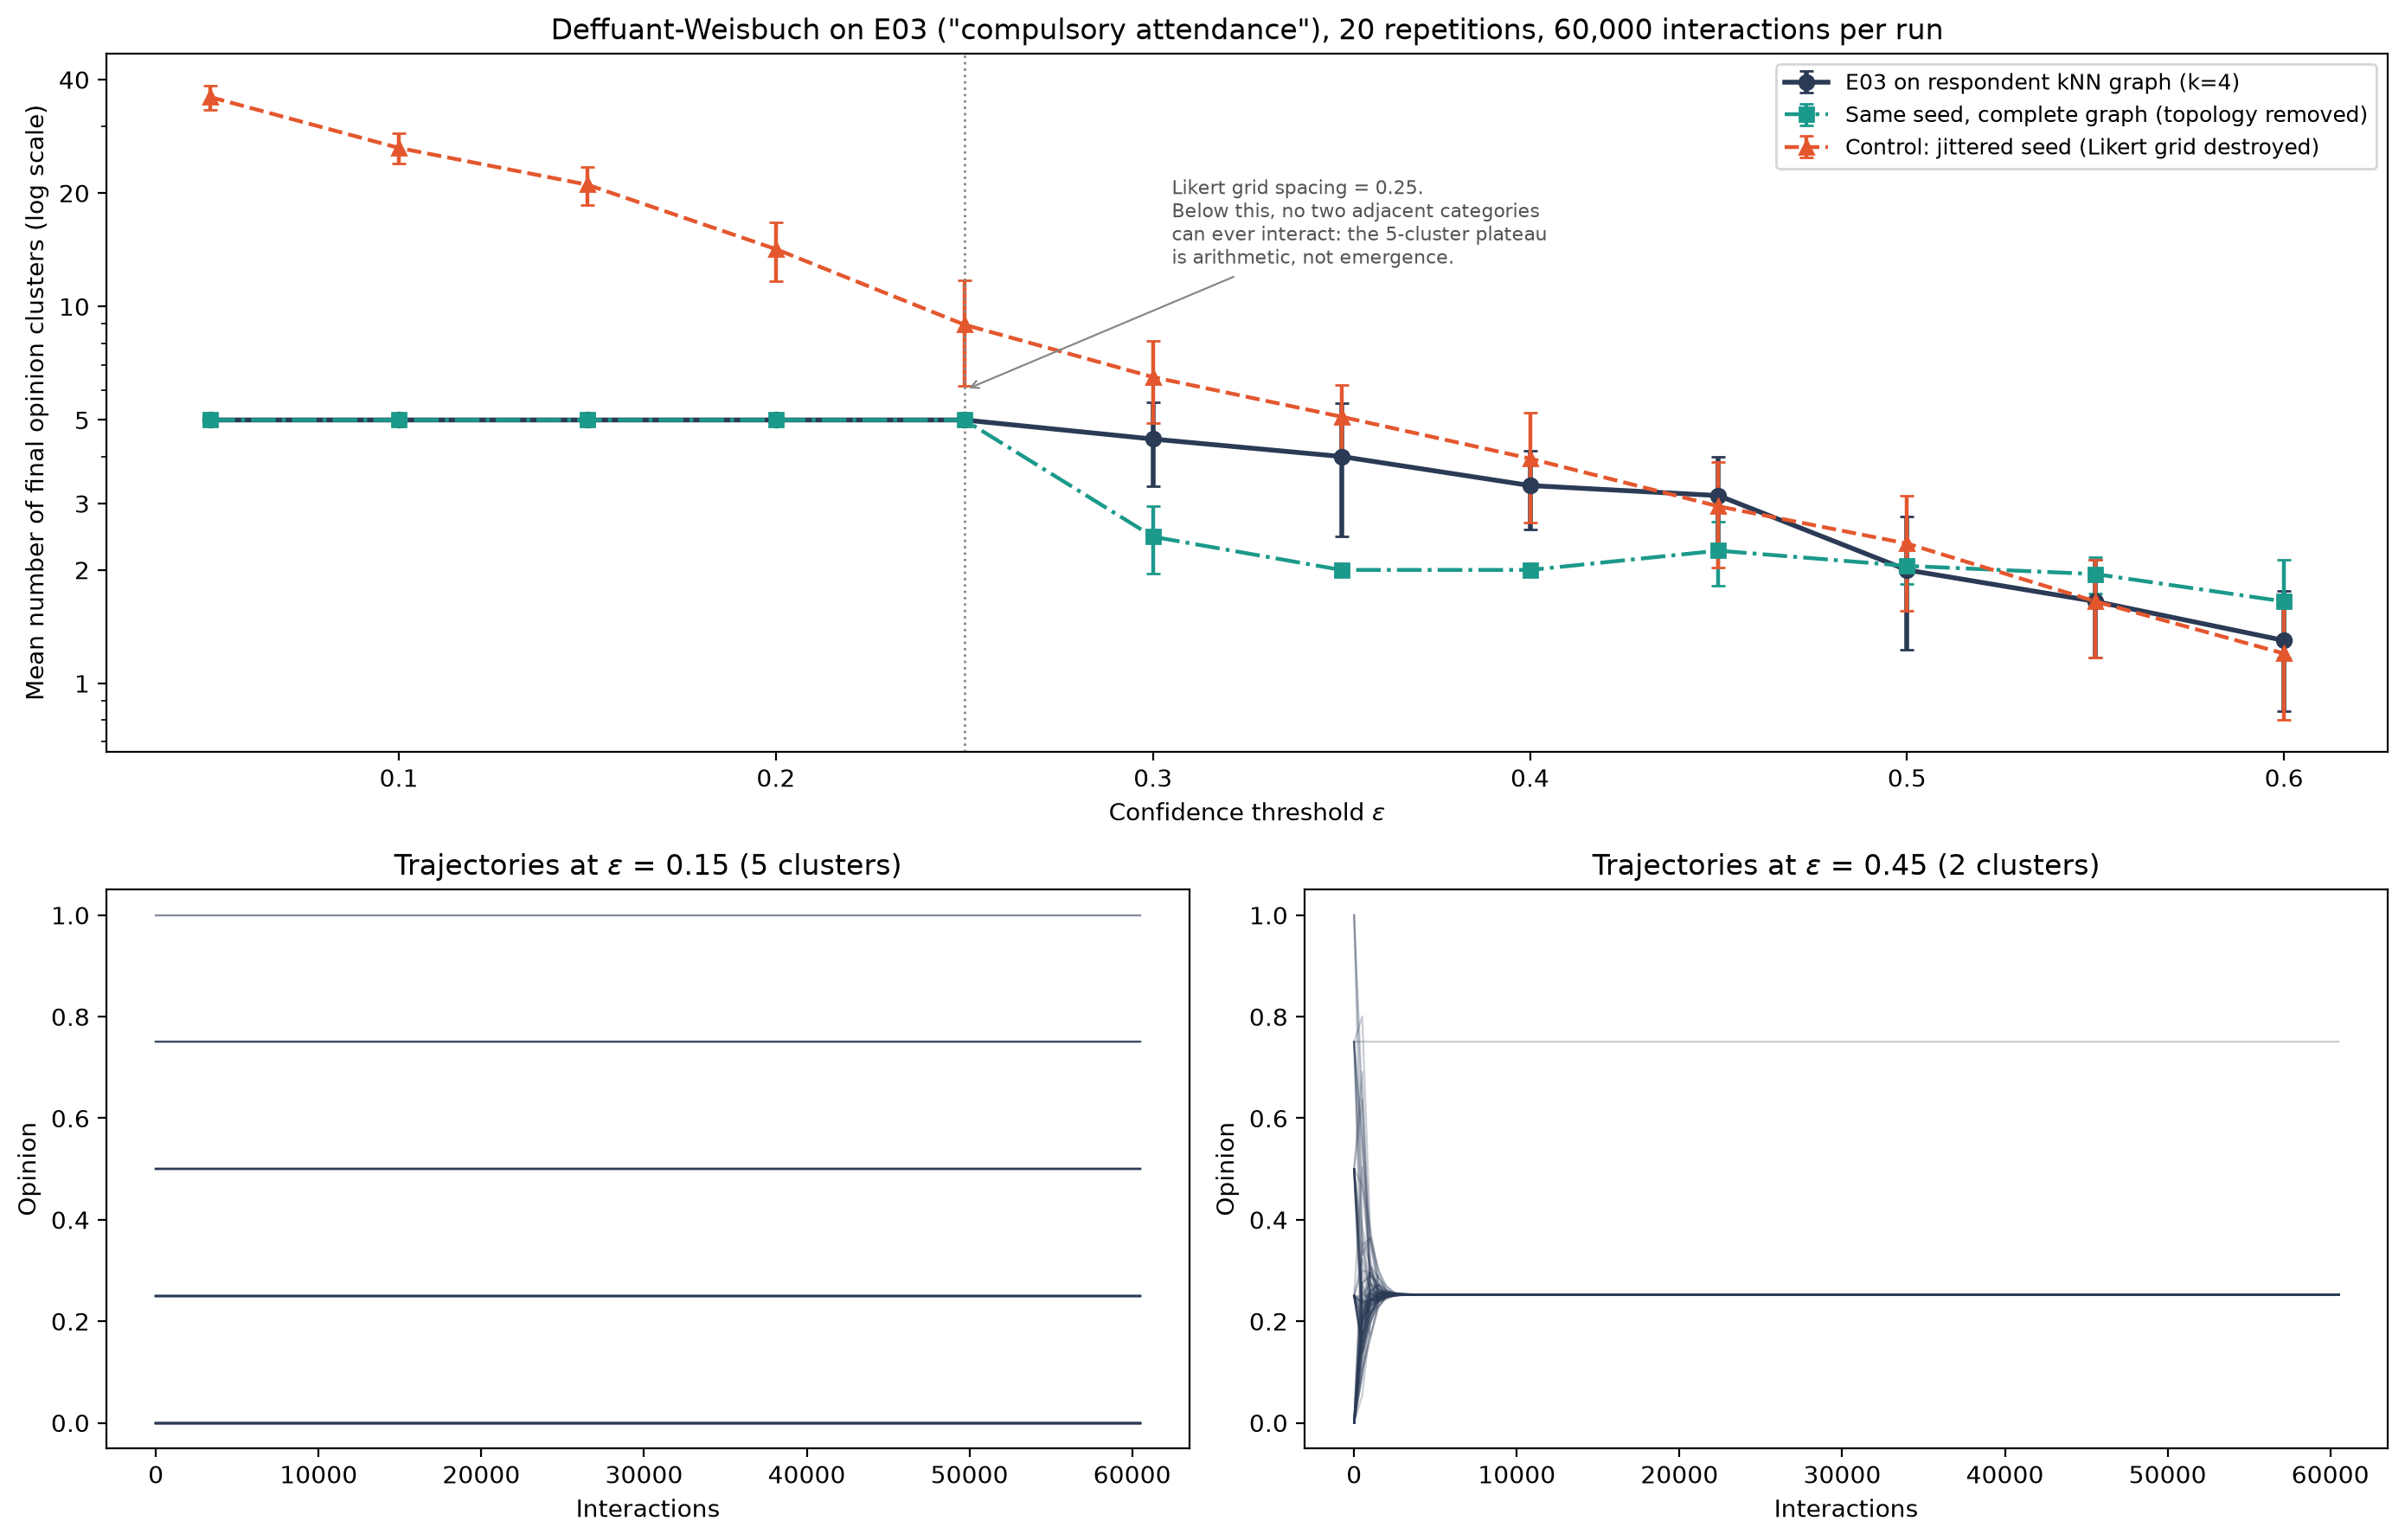
\includegraphics[width=\linewidth]{../figures/graph12_deffuant_weisbuch.png}
\caption{Top: mean final cluster count versus confidence threshold, with
error bars over 20 repetitions, on a log scale (the control curve spans an
order of magnitude more than the others). Bottom: individual opinion
trajectories at a low and a high $\varepsilon$.}
\end{figure}

\section{The small-$\varepsilon$ plateau is an artefact, and here is the proof}

The specification requires stating explicitly that the five-cluster plateau at
small $\varepsilon$ is partly an artefact of Likert responses starting on a
discrete five-point grid. In this project the claim can be made stronger than
``partly'': it is \emph{entirely} forced, and provably so.

\begin{proposition}
Under the rescaling $s(x) = (x+2)/4$, the five Likert categories map to
$\{0,\ \tfrac14,\ \tfrac12,\ \tfrac34,\ 1\}$, so any two distinct initial
opinions satisfy $|x_u - x_v| \ge \tfrac14$. For any $\varepsilon \le 0.25$
the bounded-confidence condition $|x_u - x_v| < \varepsilon$ is therefore
never satisfied by a pair with distinct opinions. The initial state is a fixed
point, and the final cluster count equals the number of occupied categories
(five) with probability one --- on \emph{any} graph.
\end{proposition}

Three independent observations confirm this empirically:

\begin{enumerate}
  \item \textbf{Zero variance.} The plateau reads $5.00 \pm 0.00$ across 20
        randomly seeded repetitions. A genuine emergent dynamical outcome
        would not be that deterministic; a frozen initial condition is.
  \item \textbf{Topology-independence.} The complete graph -- a maximally
        different topology -- produces the identical $5.00 \pm 0.00$ over the
        same range, exactly as the proposition predicts.
  \item \textbf{The control kills it.} Re-running with seeds jittered by
        $\pm 0.125$ (which destroys the grid while preserving the
        distribution's shape) removes the plateau entirely: cluster counts
        become $35.95 \to 26.35 \to 21.05 \to 14.20 \to 8.95$ across
        $\varepsilon = 0.05 \ldots 0.25$, decaying smoothly instead of
        sitting flat at five.
\end{enumerate}

So the five clusters below $\varepsilon = 0.25$ are the original response
categories failing to merge, not opinion groups forming. The figure should not
be read as showing stable pluralism at low tolerance. Note also that the
first \emph{real} dynamical behaviour begins at exactly the first swept value
above the grid spacing, $\varepsilon = 0.30$ --- the break in the curve is
arithmetic, not a discovered threshold.

\section{The network is not incidental}

Because the plateau is an artefact, the substantive dynamical result lies
above $\varepsilon = 0.25$, and it emerges from comparing the real network
against a complete graph seeded identically (i.e.\ the same dynamics with
network structure removed, a well-mixed population).

In the range $\varepsilon = 0.30$--$0.45$ the well-mixed population collapses
to about 2 clusters, while the sparse $k$NN network sustains 3.15--4.45. The
network structure therefore \emph{sustains opinion diversity that a well-mixed
population loses at the same tolerance}: when respondents only talk to their
four nearest neighbours in opinion space, locally cohesive groups stabilise
before global consensus can propagate.

This is the one result in this figure that is neither an artefact of the
response scale nor a restatement of the input distribution, and it is the
result that justifies studying the process \emph{on a network} rather than in
a well-mixed population.

\section{Artifacts}

\begin{center}
\begin{tabularx}{\linewidth}{l Y}
\toprule
Artifact & Role \\
\midrule
\texttt{outputs/sanitised\_data/row\_centred\_data.csv} & Input: row-centred matrix the respondent graph is built from \\
\texttt{outputs/sanitised\_data/dataset\_imputed.csv} & Input: uncentred matrix supplying the \texttt{E03} seed opinions \\
\texttt{src/loader.py} & \texttt{parse\_question\_columns} for item-code recovery \\
\texttt{src/dynamics.py} & New module: graph construction, DW simulation, sweep, figure \\
\texttt{figures/graph12\_deffuant\_weisbuch.png/.pdf} & The figure \\
\texttt{outputs/dynamics/dw\_sweep\_knn.csv} & Main sweep results \\
\texttt{outputs/dynamics/dw\_sweep\_control\_jittered.csv} & Control sweep (artefact demonstration) \\
\texttt{outputs/dynamics/dw\_sweep\_complete\_graph.csv} & Complete-graph comparison \\
\texttt{outputs/dynamics/respondent\_knn\_graph.edgelist} & The respondent graph, exported for reuse \\
\bottomrule
\end{tabularx}
\end{center}

The respondent graph is written out deliberately: it is the missing input for
every other respondent-level figure in the project, so exporting it means the
next such figure does not have to rebuild it.

\end{document}
